\uuid{lMbg}
\exo7id{7050}
\titre{exo7 7050}
\auteur{megy}
\organisation{exo7}
\datecreate{2017-01-08}
\isIndication{false}
\isCorrection{true}
\chapitre{Géométrie affine euclidienne}
\sousChapitre{Géométrie affine euclidienne du plan}
\module{Géométrie}
\niveau{L2}
\difficulte{}

\contenu{
\texte{
Soit $ADC$ un triangle équilatéral et $B$ le symétrique de $A$ par rapport à $D$. Montrer que $ABC$ est rectangle en $C$ et déterminer également $\widehat A$ et $\widehat B$.
\begin{center}
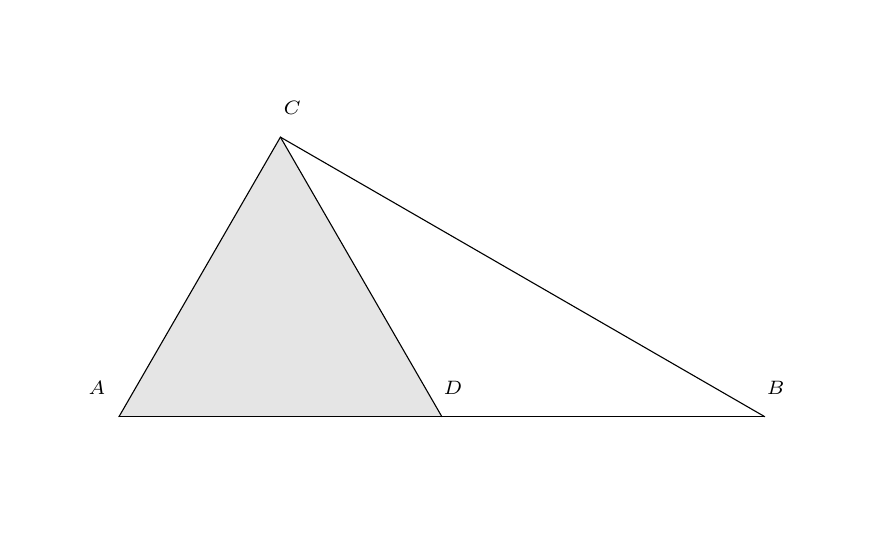
\begin{tikzpicture}[line cap=round,line join=round,x=1.0cm,y=1.0cm]
\clip(-1.38,-0.88) rectangle (9.2,5.2);
\fill[fill opacity=0.1] (-0.22,0.26) -- (3.88,0.26) -- (1.83,3.81) -- cycle;
\draw  (-0.22,0.26)-- (3.88,0.26);
\draw  (3.88,0.26)-- (1.83,3.81);
\draw  (1.83,3.81)-- (-0.22,0.26);
\draw (7.98,0.26)-- (1.83,3.81);
\draw (7.98,0.26)-- (3.88,0.26);
\begin{scriptsize}
\draw (-0.5,0.62) node {$A$};
\draw (4.02,0.62) node {$D$};
\draw (1.98,4.18) node {$C$};
\draw (8.12,0.62) node {$B$};
\end{scriptsize}
\end{tikzpicture}
\end{center}
}
\reponse{
Comme par hypoth\`ese $DA = DC = DB$, les points $A$, $B$ et $C$ sont situés sur le cercle de centre $A$ et de diam\`etre $AB$. Donc, $ACB$ est rectangle en $C$. 

\begin{center}
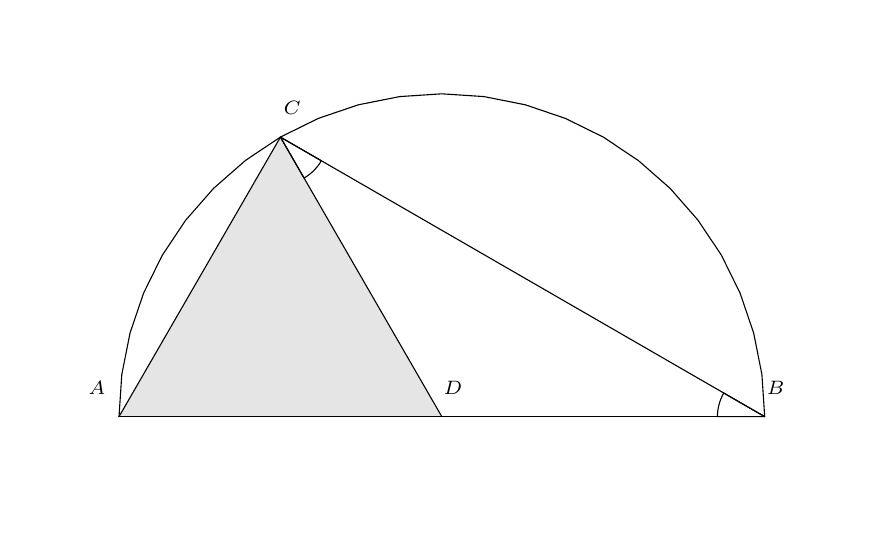
\begin{tikzpicture}[line cap=round,line join=round,x=1.0cm,y=1.0cm]
\clip(-1.38,-0.88) rectangle (9.2,5.2);
\fill[fill opacity=0.1] (-0.22,0.26) -- (3.88,0.26) -- (1.83,3.81) -- cycle;
\draw [shift={(1.83,3.81)},fill opacity=0.1] (0,0) -- (-60.:0.6) arc (-60.:-30.:0.6) -- cycle;
\draw [shift={(7.98,0.26)},fill opacity=0.1] (0,0) -- (150.:0.6) arc (150.:180.:0.6) -- cycle;
\draw  (-0.22,0.26)-- (3.88,0.26);
\draw  (3.88,0.26)-- (1.83,3.81);
\draw  (1.83,3.81)-- (-0.22,0.26);
\draw (7.98,0.26)-- (1.83,3.81);
\draw (7.98,0.26)-- (3.88,0.26);
\draw [shift={(3.88,0.26)}] plot[domain=0.:3.141592653589793,variable=\t]({1.*4.1*cos(\t r)+0.*4.1*sin(\t r)},{0.*4.1*cos(\t r)+1.*4.1*sin(\t r)});
\begin{scriptsize}
\draw (-0.5,0.62) node {$A$};
\draw (4.02,0.62) node {$D$};
\draw (1.98,4.18) node {$C$};
\draw (8.12,0.62) node {$B$};
\end{scriptsize}
\end{tikzpicture}
\end{center}

Puisque $ADC$ est équilatéral, $\widehat{DAC} = \widehat{BAC}= 60^{\circ}$. Comme $ACB$ est rectangle en $C$, donc $\widehat{ACB}=90^{\circ}$.

De la relation $180^{\circ} = \widehat{BAC} + \widehat{ACB} + \widehat{CBA}$ on tire $\widehat{CBA} = 30^{\circ}$.
}
}
